\documentclass[openbib]{article}

\usepackage{color}
\usepackage{ctex}
\usepackage{mathtools}
\usepackage{amsmath}
\usepackage{graphicx,psfrag,epsfig}
\usepackage{float}

\usepackage{fontspec}
\usepackage{bm}
\graphicspath{{figures/}}
\renewcommand{\contentsname}{\centerline{目录}}

\usepackage{multirow}
\begin{document}
	\title{Jetson Nano Developer Kit}
	
	\maketitle
	
	\newpage
	\tableofcontents
	\newpage
	
\section{设备介绍}
NVIDIA® Jetson Nano™ 开发人员套件是一款面向创客、学习者和开发人员的小型 AI 计算机。

遵循本简要指南后,您就可以开始构建实用的 AI 应用程序、酷炫的 AI 机器人等。
\begin{figure}[htbp]
	\centering
	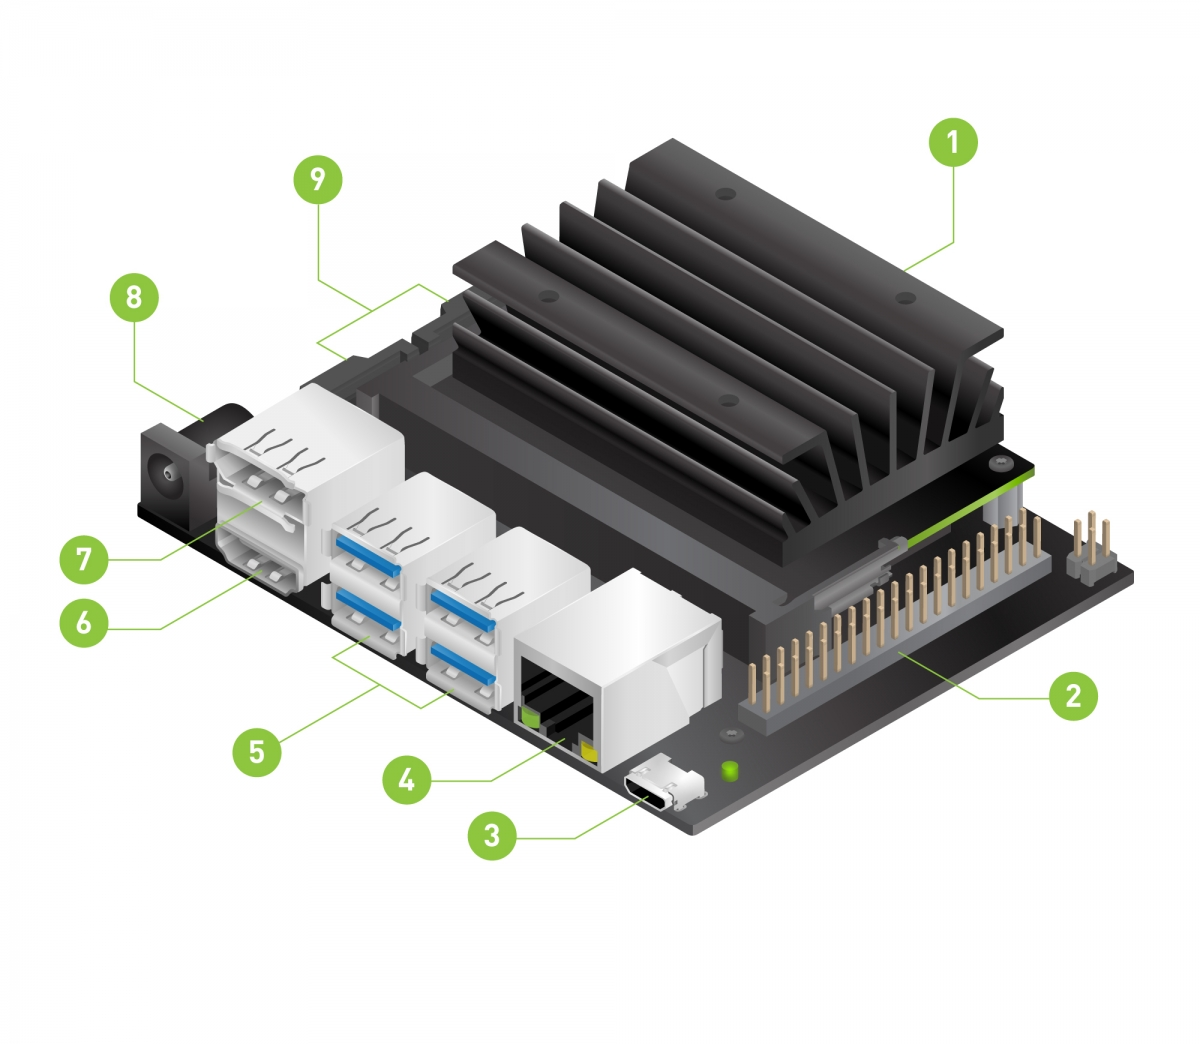
\includegraphics[scale=0.4]{1}
\end{figure}	

上图标号:

1.用于主存储的 microSD 卡插槽

2.40针扩展接头

3.用于5V电源输入或设备模式的微型USB端口(一般不用此口作为电源输入)

4.千兆网口

5.USB 3.0 端口 (x4)

6.HDMI输出端口

7.显示端口连接器

8.用于5V电源输入的DC桶形插孔

9.MIPI CSI-2 摄像头连接器
\section{将镜像文件写入sd卡中}
Jetson Nano Developer Kit使用microSD卡作为启动设备和主存储。容量是64GB UHS-1 卡。
\subsection{镜像文件下载与解压}
1.从https://developer.nvidia.com/jetson-nano-sd-card-image下载 Jetson Nano Developer Kit SD卡映像压缩包,并记下它在计算机上的保存位置。
\begin{figure}[htbp]
	\centering
	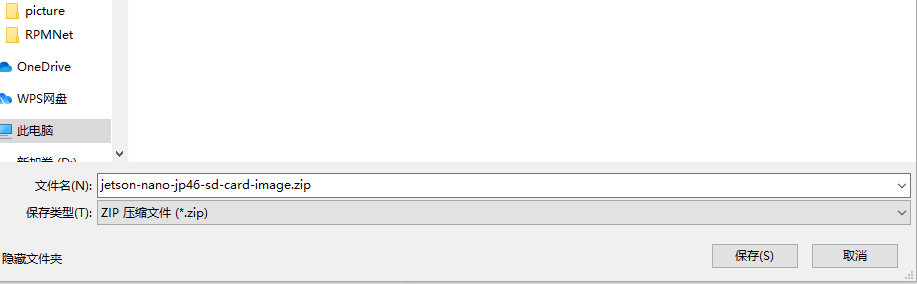
\includegraphics[scale=0.4]{image}
\end{figure}

2.打开我的电脑找到所下载压缩包的位置,进行解压操作。解压完能看到以下的文件。
\begin{figure}[htbp]
	\centering
	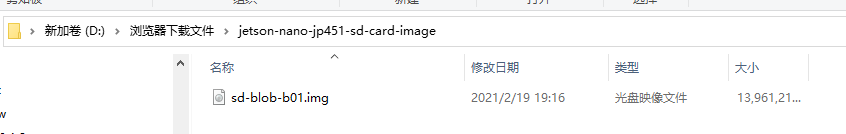
\includegraphics[scale=0.4]{a1}
\end{figure}

3.记住该位置
\subsection{相关软件下载与安装}
\subsubsection{安装SD Card Formatter}
使用SD协会的SD存储卡格式化程序格式化您的 microSD 卡。

1.进入以下网站:(https://www.sdcard.org/downloads/formatter\_4/eula\_windows/),将网页拉到最底下,点击accept。进行文件下载。
\begin{figure}[htbp]
	\centering
	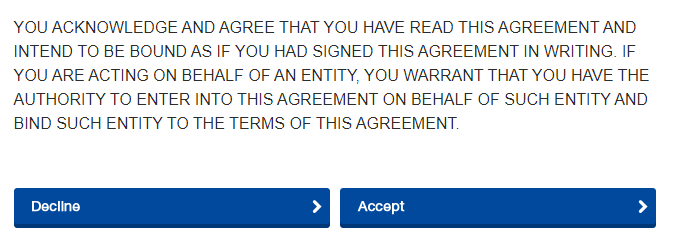
\includegraphics[scale=0.3]{a2}
\end{figure}


2.将压缩包解压缩之后,能得到exe文件进行双击进行安装。点击Next,进行下一步安装。
\begin{figure}[htbp]
	\centering
	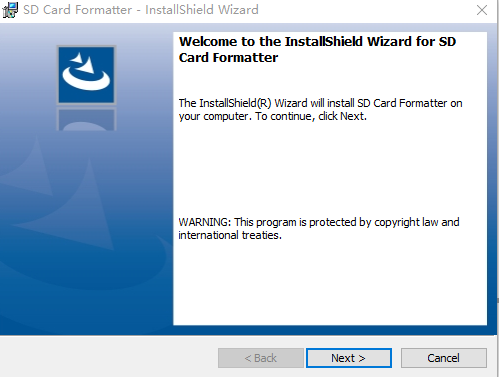
\includegraphics[scale=0.3]{a3}
\end{figure}

3.选择接受条款,点击Next,进行下一步安装。
\begin{figure}[H]
	\centering
	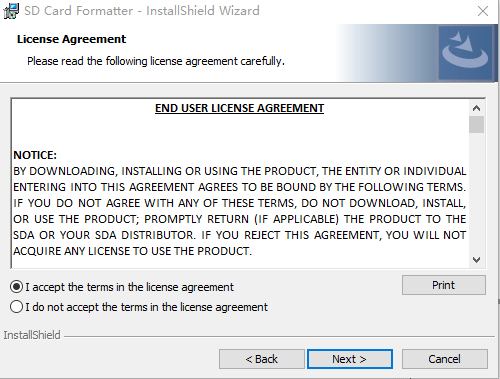
\includegraphics[scale=0.4]{a4}
\end{figure}

4.选择想安装到的文件夹,点击Next。
\begin{figure}[H]
	\centering
	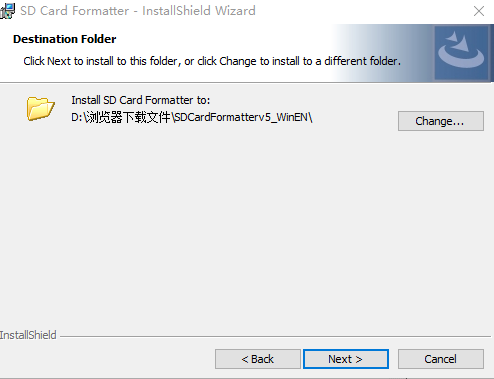
\includegraphics[scale=0.4]{a5}
\end{figure}

5.安装信息确定,确定无误后点击install
\begin{figure}[H]
	\centering
	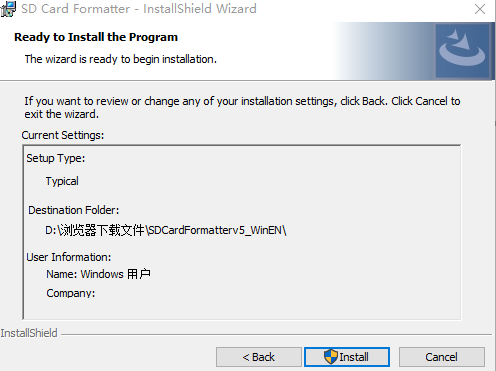
\includegraphics[scale=0.35]{a6}
\end{figure}

6.等待
\begin{figure}[H]
	\centering
	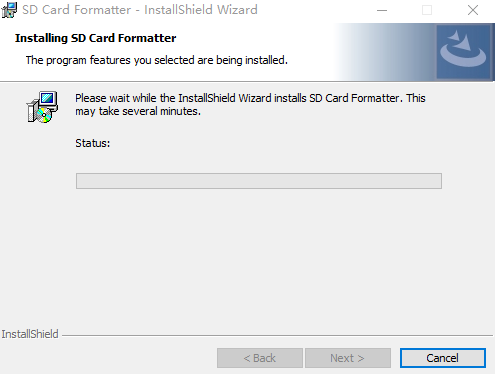
\includegraphics[scale=0.35]{a7}
\end{figure}

7.安装完成,点击finish,运行程序
\begin{figure}[H]
	\centering
	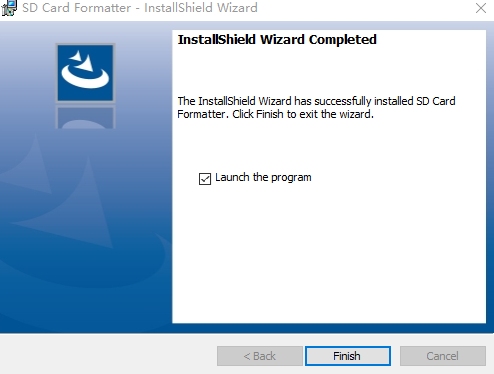
\includegraphics[scale=0.35]{a8}
\end{figure}

8.运行界面如下
\begin{figure}[H]
	\centering
	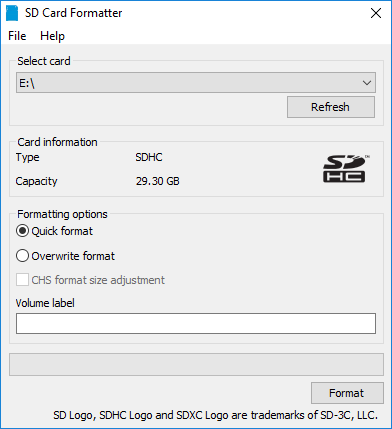
\includegraphics[scale=0.4]{SD Card Formatter}
\end{figure}

\subsubsection{安装Etcher}
使用 Etcher 将 Jetson Nano Developer Kit SD 卡映像写入您的 microSD 卡

1.进入以下的网站(https://www.balena.io/etcher)进行下载。


2.将网站拉下一点点,看到以下界面
\begin{figure}[H]
	\centering
	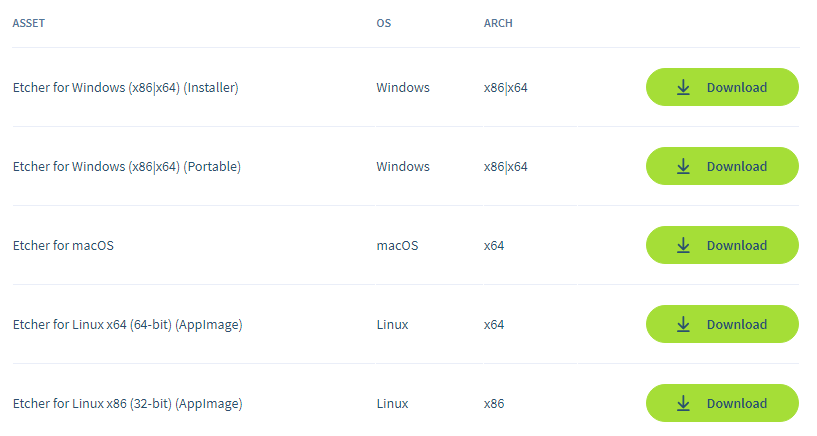
\includegraphics[scale=0.35]{b1}
\end{figure}

3.点击第一个的下载按钮,可以下载一个exe文件

4.打开我的电脑,到你下载的文件的路径下,双击运行该文件。

5.点击我同意
\begin{figure}[H]
	\centering
	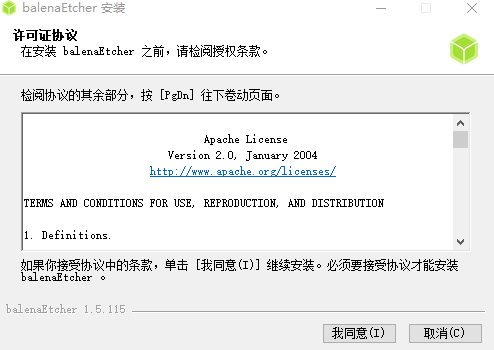
\includegraphics[scale=0.35]{b2}
\end{figure}

6.等待安装,之后就能出现下面的界面

\begin{figure}[H]
	\centering
	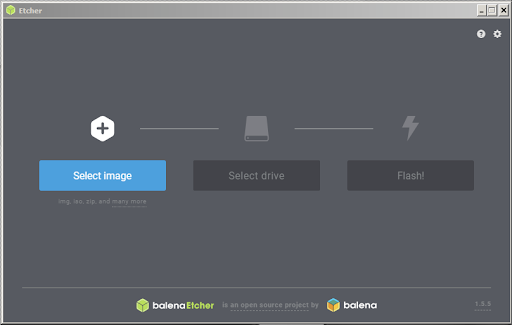
\includegraphics[scale=0.4]{Etcher}
\end{figure}

\subsection{制作启动盘}
将sd卡如下图所示插入读卡器,再将读卡器插入电脑中。

\begin{figure}[H]
	\centering
	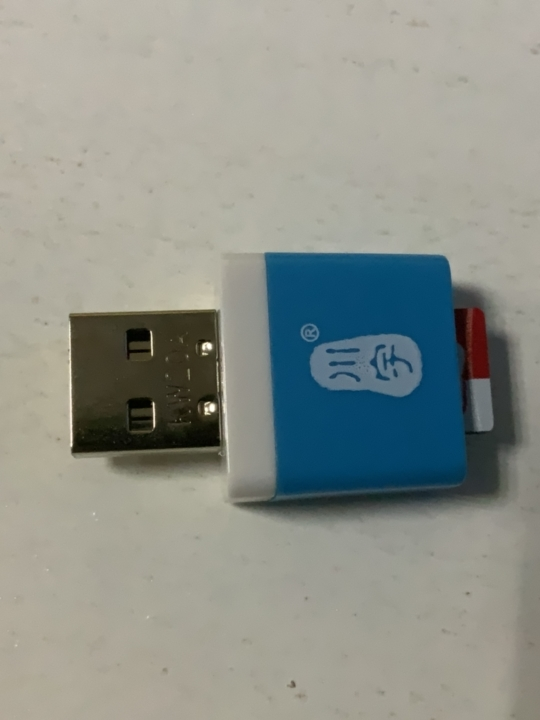
\includegraphics[scale=0.2]{a9}
\end{figure}

1.先打开SD Card Formatter软件,选择插入sd卡的盘符,选择"Quick format","Volume label"不填。如下图

\begin{figure}[H]
	\centering
	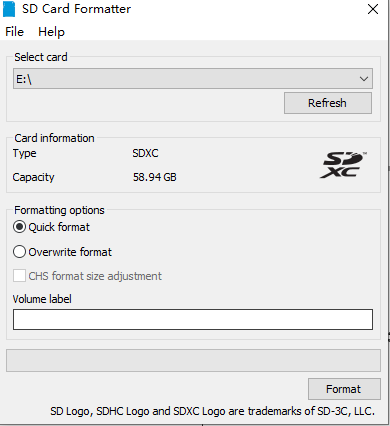
\includegraphics[scale=0.4]{b3}
\end{figure}


5.单击“Format”开始格式化,然后在警告对话框中单击“是”

\begin{figure}[H]
	\centering
	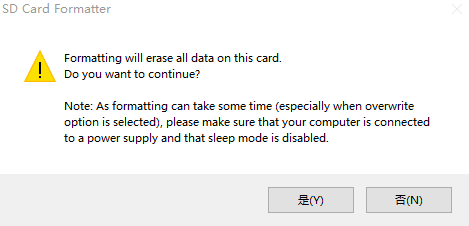
\includegraphics[scale=0.4]{b4}
\end{figure}

6.格式化完后,会显示出相关信息.点击确定。关闭软件

\begin{figure}[H]
	\centering
	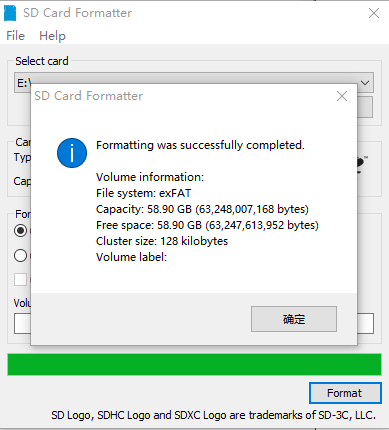
\includegraphics[scale=0.4]{b5}
\end{figure}

7.打开Etcher,选择flash from file.
\begin{figure}[H]
	\centering
	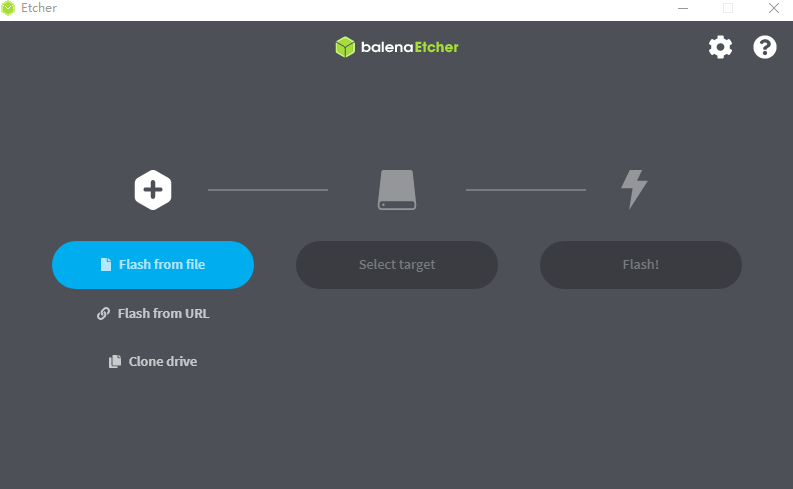
\includegraphics[scale=0.4]{b6}
\end{figure}

8.选择解压出来的镜像文件
\begin{figure}[H]
	\centering
	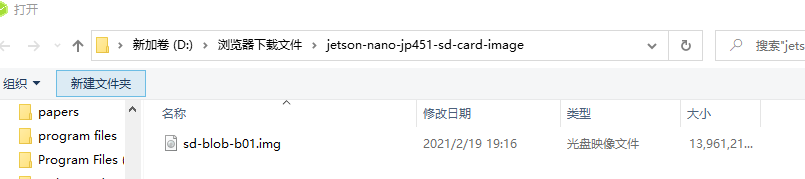
\includegraphics[scale=0.4]{b7}
\end{figure}

9.选择 select target
\begin{figure}[H]
	\centering
	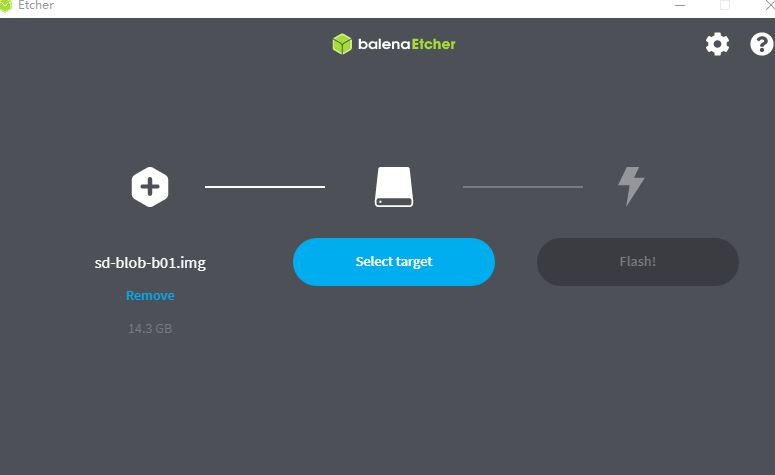
\includegraphics[scale=0.4]{b8}
\end{figure}

10.选择要写入的sd卡,点击select
\begin{figure}[H]
	\centering
	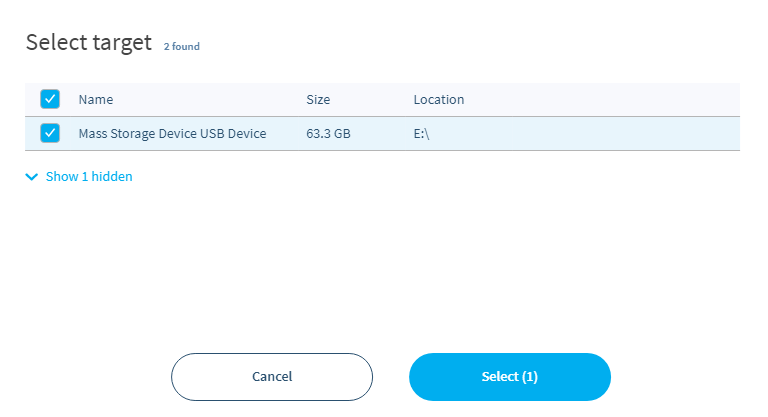
\includegraphics[scale=0.4]{b9}
\end{figure}

11.点击flash!
\begin{figure}[H]
	\centering
	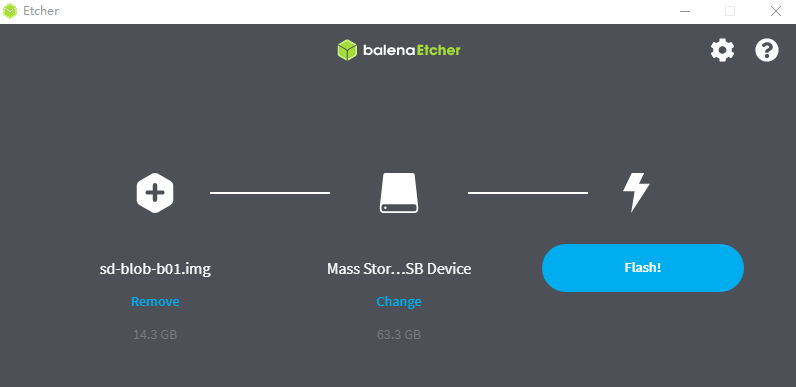
\includegraphics[scale=0.4]{b10}
\end{figure}

12.等待。
\begin{figure}[H]
	\centering
	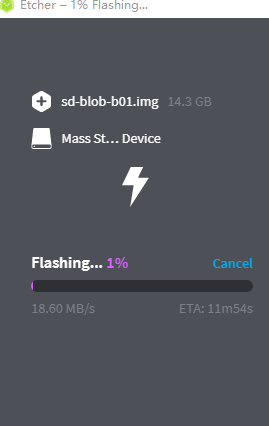
\includegraphics[scale=0.4]{b11}
\end{figure}

13.Etcher 完成后,Windows可能会让您知道它不知道如何读取SD卡。只需单击取消并电脑中弹出读卡器,拔出读卡器,取出 microSD 卡即可。
\begin{figure}[H]
	\centering
	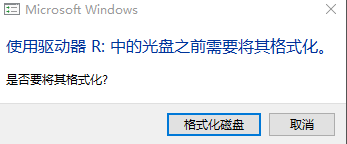
\includegraphics[scale=0.4]{b12}
\end{figure}
\section{设置和首次启动}
1.将sd卡从读卡器中取出,插入Jetson Nano模块底部的插槽中。

\begin{figure}[htbp]
	\centering
	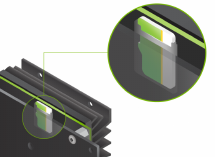
\includegraphics[scale=0.3]{sd}
\end{figure}

2.连接显示器和USB的鼠标和键盘

3.插上电源(请见设备介绍有说明,一般使用5vDC电源)。特别注意:设备默认为USB端口供电,要使用DC电源供电,需要杜邦线或跳线棒短接USB端口,在DC电源口上方,如图:
\begin{figure}[H]
	\centering
	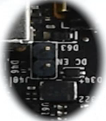
\includegraphics[scale=0.3]{souce}
\end{figure}

4.一旦开发人员套件通电,Micro-USB 连接器旁边的绿色 LED 就会亮起。当您第一次启动时,开发人员工具包将引导您完成一些初始设置
\subsection{初始化设置}
1.System Configuration(选择接受条款,点击继续)
\begin{figure}[htbp]
	\centering
	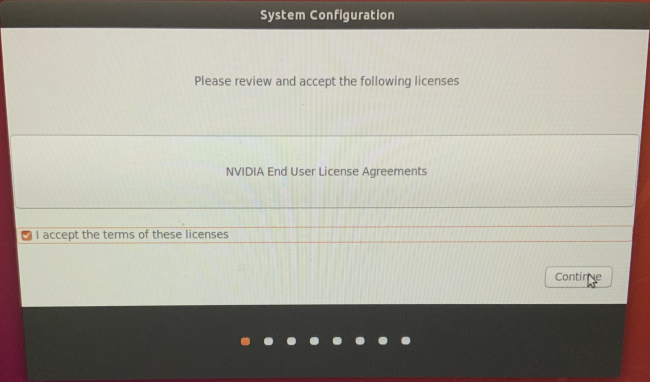
\includegraphics[scale=0.3]{01}
\end{figure}

2.语言设置
\begin{figure}[H]
	\centering
	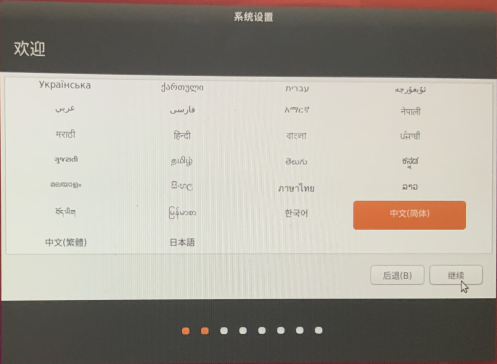
\includegraphics[scale=0.3]{02}
\end{figure}

3.键盘设置
\begin{figure}[H]
	\centering
	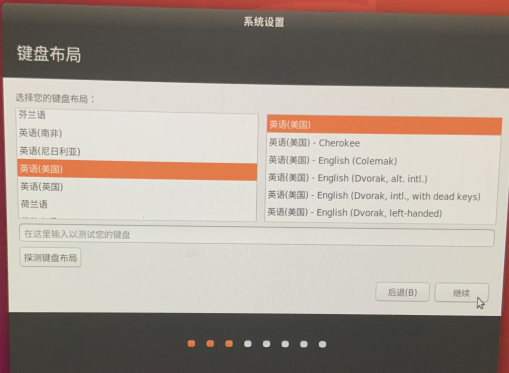
\includegraphics[scale=0.3]{03}
\end{figure}

4.地域设置
\begin{figure}[H]
	\centering
	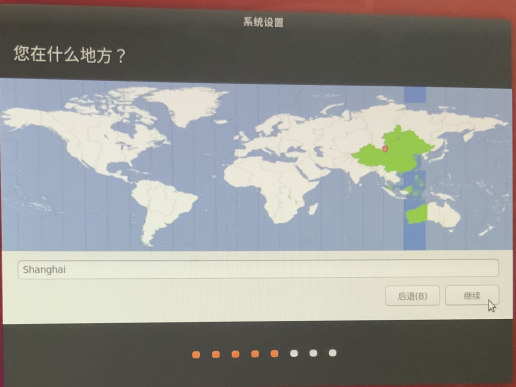
\includegraphics[scale=0.3]{04}
\end{figure}

5.系统设置
\begin{figure}[H]
	\centering
	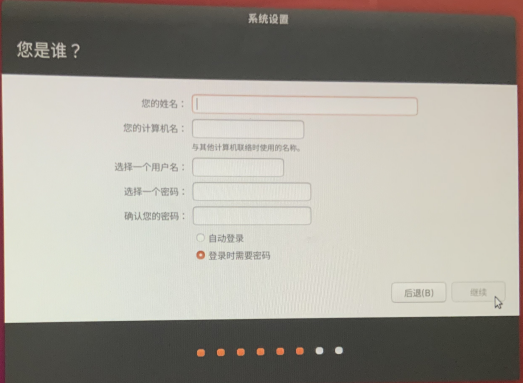
\includegraphics[scale=0.3]{06}
\end{figure}

6.存储大小设置
\begin{figure}[H]
	\centering
	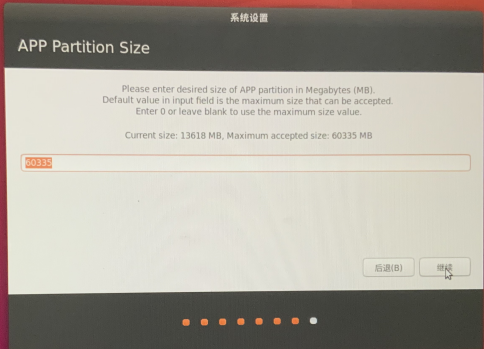
\includegraphics[scale=0.3]{05}
\end{figure}

7.模式选择,继续。
\begin{figure}[H]
	\centering
	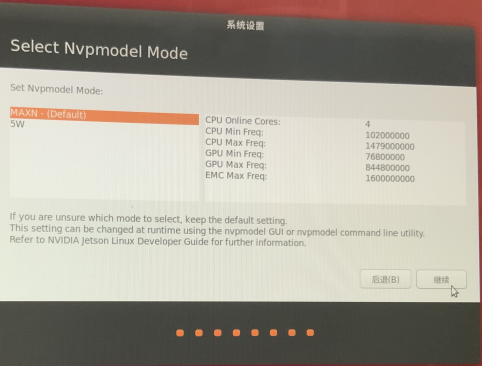
\includegraphics[scale=0.3]{07}
\end{figure}

8.等待安装
\begin{figure}[H]
	\centering
	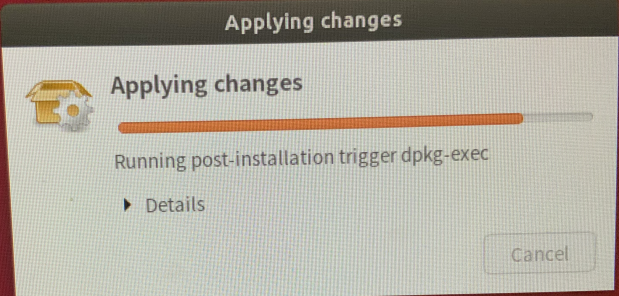
\includegraphics[scale=0.3]{c1}
\end{figure}

9.完成了系统的安装,打密码后进入系统。
\begin{figure}[H]
	\centering
	
\includegraphics[scale=0.3]{c2}
\end{figure}
\section{安装依赖包}
\subsection{准备python环境}
1.更新

进入操作系统页面,调出终端,输入指令

sudo apt-get update

\begin{figure}[H]
	\centering
	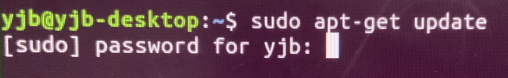
\includegraphics[scale=0.3]{c3}
\end{figure}

要你输入设置的密码,且你输入时不是显式显现的。

完成后,再输入以下指令

sudo apt-get upgrade

\begin{figure}[H]
	\centering
	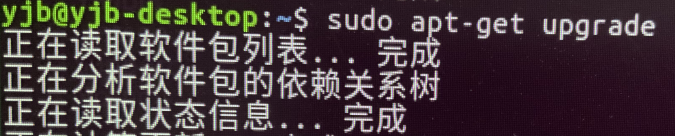
\includegraphics[scale=0.3]{c4}
\end{figure}
会询问你是否要继续执行,输入y,后回车
\begin{figure}[H]
	\centering
	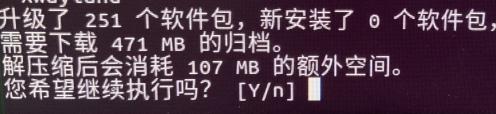
\includegraphics[scale=0.3]{c5}
\end{figure}
2.安装所需要的包

sudo apt-get install git cmake python3-dev
\begin{figure}[H]
	\centering
	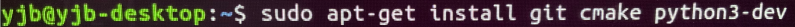
\includegraphics[scale=0.3]{d1}
\end{figure}

sudo apt-get install libhdf5-serial-dev hdf5-tools libhdf5-dev zlib1g-dev zip libjpeg8-dev

\begin{figure}[H]
	\centering
	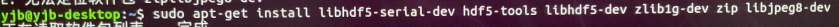
\includegraphics[scale=0.3]{d2}
\end{figure}

sudo apt-get install python3-pip

\begin{figure}[H]
	\centering
	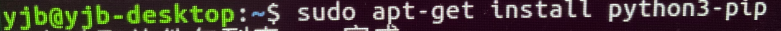
\includegraphics[scale=0.3]{d3}
\end{figure}
sudo pip3 install -U pip testresources setuptools
\begin{figure}[H]
	\centering
	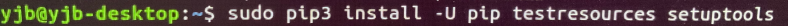
\includegraphics[scale=0.3]{d4}
\end{figure}
\subsection{安装Pytorch}
1.安装好Pytorch所需的包

sudo apt-get install libopenblas-base libopenmpi-dev
\begin{figure}[H]
	\centering
	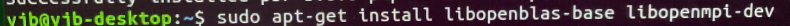
\includegraphics[scale=0.3]{d5}
\end{figure}

2.下载Pytorch的whl文件,注意一定要下后缀名为linux\_aarch64.whl。官网提供下载(https://forums.developer.nvidia.com/t/pytorch-for-jetson-version-1-9-0-now-available/72048)

3.之后在下载下来文件的路径打开终端,安装whl文件

sudo pip3 install torch-1.6.0-cp36-cp36m-linux\_aarch64.whl 
\begin{figure}[H]
	\centering
	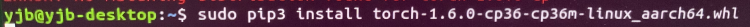
\includegraphics[scale=0.3]{d6}
\end{figure}

\subsection{安装Torchvision}
1.注意下表的对应关系,到github上下载对应的torchvision

(https://github.com/pytorch/vision/tree/master)
\begin{figure}[H]
	\centering
	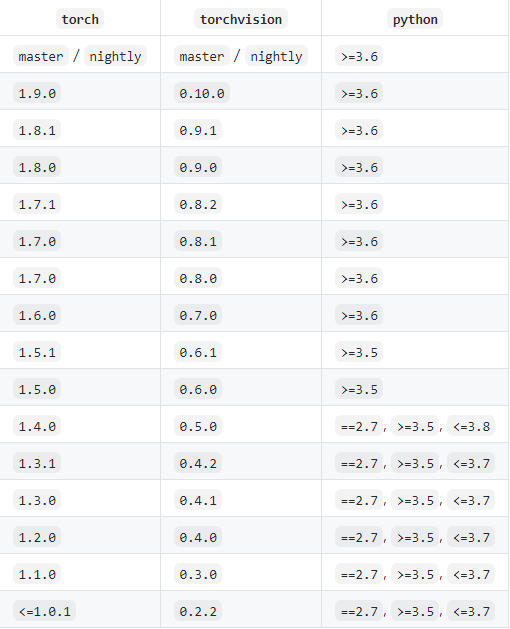
\includegraphics[scale=0.3]{torch}
\end{figure}

2.下载完成后,解压,进入解压后的目录,在此处打开终端,依次输入:

sudo apt install libavcodec-dev
\begin{figure}[H]
	\centering
	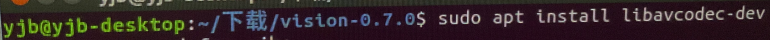
\includegraphics[scale=0.3]{d7}
\end{figure}

sudo apt install libavformat-dev

\begin{figure}[H]
	\centering
	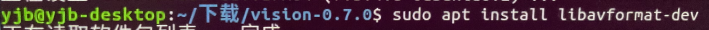
\includegraphics[scale=0.3]{d8}
\end{figure}

sudo apt install libswscale-dev
\begin{figure}[H]
	\centering
	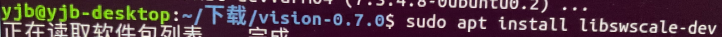
\includegraphics[scale=0.3]{d9}
\end{figure}

sudo python3 setup.py install
\begin{figure}[H]
	\centering
	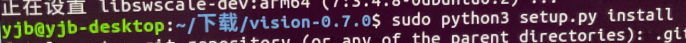
\includegraphics[scale=0.3]{d10}
\end{figure}

3.最后也能输入指令看看是否安装成功,从终端进入python3。依次输入以下指令:

import torch

import torchvision

print(torch.\_\_version\_\_)

print(torchvision.\_\_version\_\_)

看看安装的版本号。

\subsection{安装torch2trt}
1.下载源代码(https://github.com/NVIDIA-AI-IOT/torch2trt)

2.下载完成后,解压,进入解压后的目录,在此处打开终端,输入代码:

sudo python3 setup.py install $--$plugins
\begin{figure}[H]
	\centering
	\includegraphics[scale=0.3]{d11}
\end{figure}

\subsection{安装trt\_pose}
1.下载源代码(https://github.com/NVIDIA-AI-IOT/trt\_pose)

2.下载完成后,解压,进入解压后的目录,在此处打开终端,输入代码:

sudo python3 setup.py install 
\begin{figure}[H]
	\centering
	\includegraphics[scale=0.3]{d12}
\end{figure}
%\subsection{安装其他杂项包}
%sudo pip3 install tqdm cython pycocotools

%sudo apt-get install python3-matplotlib

\subsection{安装Jupyter lab}
1.先安装一些依赖的包

sudo apt install nodejs npm
\begin{figure}[H]
	\centering
	\includegraphics[scale=0.3]{d13}
\end{figure}

sudo pip3 install pillow
\begin{figure}[H]
	\centering
	\includegraphics[scale=0.3]{d14}
\end{figure}
2.安装jupyter lab

pip3 install jupyter jupyterlab
\begin{figure}[H]
	\centering
	\includegraphics[scale=0.3]{d15}
\end{figure}
3.重启设备

sudo reboot
\begin{figure}[H]
	\centering
	\includegraphics[scale=0.3]{d16}
\end{figure}
4.启动jupyter lab

在命令行中输入jupyter lab命令,即可以启动jupyter lab

\section{配置运行环境}
1.打开本地的文件夹中的/Home目录,找到.bashrc(该文件为隐藏文件),打开。

\begin{figure}[H]
	\centering
	\includegraphics[scale=0.3]{d17}
\end{figure}
2.在该文件中加入以下命令

export CUDA\_HOME=/usr/local/cuda-10.2

export LD\_LIBRARY\_PATH=/usr/local/cuda-10.2/lib64:\$LD\_LIBRARY\_PATH

export PATH=/usr/local/cuda-10.2/bin:\$PATH

export LD\_PRELOAD=/usr/lib/aarch64-linux-gnu/libgomp.so.1:\$LD\_PRELOAD
\begin{figure}[H]
	\centering
	\includegraphics[scale=0.3]{b13}
\end{figure}
3.保存,关闭,更新当前终端上的配置,命令行输入

source ~/.bashrc
\begin{figure}[H]
	\centering
	\includegraphics[scale=0.3]{b14}
\end{figure}
\end{document}